\documentclass[../../main.tex]{subfiles}

\graphicspath{{\subfix{../../immagini/}}}

\begin{document}

\section{Descrizione della struttura}
\label{sec:BFStruttura}
Un \textit{filtro di Bloom} \cite{Bloom1970SpacetimeTI} è una struttura dati probabilistica basata su funzioni di hash, il cui obiettivo è quello di rappresentare un insieme di elementi in un modo tale da permettere di verificare se un generico elemento appartenga o meno a tale insieme. Un filtro di Bloom può generare falsi positivi, ma non falsi negativi.

Questa struttura trova il suo principale utilizzo nei contesti in cui mantenere tutto l'insieme in memoria richiederebbe molto più spazio di quello a disposizione: il filtro infatti consiste semplicemente in un array di $n$ bit, inizializzati a $0$, e una serie di $k$ funzioni di hash\footnote{Una funzione di hash è una funzione non invertibile in grado di mappare elementi di grandezza arbitraria in elementi di un sottoinsieme di grandezza prefissata.}, che mappano in modo uniforme sulle $n$ possibili posizioni. Ogni elemento appartenente all'insieme viene passato attraverso le $k$ funzioni e i bit presenti nelle posizioni restituite vengono posti ad 1. Intuitivamente, fissata la dimensione $n$ del filtro, maggiori sono gli elementi da inserire, maggiore è la probabilità di ottenere falsi positivi.

Formalmente quindi un Filtro di Bloom è formato da:
    \begin{itemize}
        \item un array di $n$ bit, inizializzati a 0,
        \item un insieme di $k$ funzioni di hash $h_1, h_2, \dots, h_k$ che restituiscono, con probabilità uniforme, una posizione tra $0$ ed $n-1$,
        \item un insieme $\mathcal{S}$ di chiavi da inserire nel filtro con $|\mathcal{S}| = m$.
    \end{itemize}
Per verificare l'appartenenza di un elemento $x$ all'insieme è quindi necessario controllare che tutti i bit nelle posizioni equivalenti ai risultati delle funzioni di hash $h_1(x), \dots h_k(x)$ abbiano valore 1: l'elemento viene indicato come appartenente all'insieme se e solo se tutte le funzioni di hash hanno valore uguale a 1. Ovviamente quindi, data la natura delle funzioni di hash, potranno essere presenti delle collisioni: più elementi possono venire mappati nella stessa posizione. Per questo motivo se, dato un generico elemento, una delle funzioni restituisce una posizione a cui è associato uno 0 si può essere certi della sua non appartenenza al filtro; viceversa, se tutte le funzioni restituiscono 1 è comunque possibile che l'elemento non appartenga all'insieme $\mathcal{S}$.

Nella Figura \ref{fig:BFExample} viene mostrato un esempio di un filtro di Bloom subito dopo la sua inizializzazione (Figura \ref{fig:BFCreazione}), subito dopo l'inserimento di tutti gli elementi in $\mathcal{S}$ (Figura \ref{fig:BF:Inizializzazione}) e durante l'operazione di controllo dell'appartenenza di un generico elemento (Figura \ref{fig:BFAppartenenza}).

\begin{figure}[H]
    \centering
    \begin{subfigure}[b]{0.70\textwidth}
       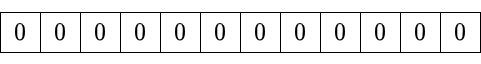
\includegraphics[width=1\linewidth]{immagini/3/bloomFilterInitial .png}
       \caption{}
       \label{fig:BFCreazione} 
    \end{subfigure}
    
    \begin{subfigure}[b]{0.70\textwidth}
       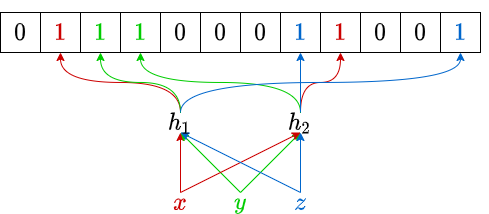
\includegraphics[width=1\linewidth]{immagini/3/bloomFilterInserimento.png}
       \caption{}
       \label{fig:BF:Inizializzazione}
    \end{subfigure}
 
    \begin{subfigure}[b]{0.70\textwidth}
        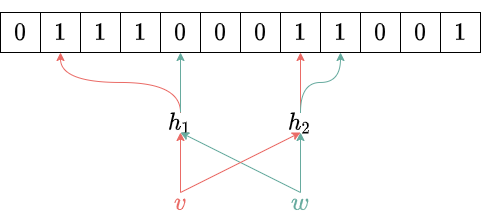
\includegraphics[width=1\linewidth]{immagini/3/bloomFilterCheck.png}
        \caption{}
        \label{fig:BFAppartenenza}
     \end{subfigure}
    \caption{Rappresentazione di un filtro di Bloom di dimensione $n=12$ basato su $k=2$ funzioni di hash: (a) subito dopo la sua inizializzazione, (b)  subito dopo l'inserimento degli elementi dell'insieme e (c) durante il controllo dell'appartenenza di due elementi $v$ e $w$ non appartenenti all'insieme di partenza. Si noti come il primo di questi elementi generi un falso positivo.}
    \label{fig:BFExample}
\end{figure}

La probabilità $f$ di ottenere un falso positivo può essere quantificata dalla formula
\begin{equation}
    f = \left(1 - \left(1 - \frac{1}{n}\right)^{km}\right)^k \approx \left(1 - e^{-km/n}\right)^k,
    \label{eqn:bloomfpr}
\end{equation}
in quanto abbiamo supposto che ogni funzione di hash mappi con probabilità uniforme su ognuno degli $n$ bit  dell'array. Di conseguenza, dato un elemento $x$ da inserire nel filtro, la probabilità che uno specifico bit non venga impostato a 1 dopo che l'elemento è passato per tutte le $k$ funzioni di hash è
\[\left(1 - \frac{1}{n}\right)^k.\]
L'inserimento deve inoltre essere effettuato per tutti gli $m \in \mathcal{S}$ elementi, supponendo ogni inserimento come un evento indipendente\footnote{Nella realtà l'indipendenza tra successivi inserimenti non vale: il fatto che un bit venga posto ad 1 influenza la probabilità degli altri bit di essere posti ad uno, di fatto quindi $e^{-km/n}$ rappresenta il valore atteso della frazione di bit a 0 dopo l'inserimento. In \cite{10.1145/383962.384004} viene però dimostrato che il valore reale di tale frazione risulta comunque altamente concentrata attorno al suo valore atteso. Nello specifico, indicata con $X$ variabile aleatoria che rappresenta il numero di bit a 0 dopo l'inserimento vale $\mathbb{P}\left(|X - m e^{-km/n}| > \epsilon m \right) < 2e^{(-\epsilon^2 n^2)/2mk}$ per ogni $\epsilon > 0$.} e $n$ sufficiente grande:
\[\left(1 - \frac{1}{n}\right)^{km} = \left(\left(1 - \frac{1}{n}\right)^n\right)^{km/n} \approx e^{-km/n},\]
di conseguenza la probabilità che un dato bit sia a 1 dopo l'inserimento di $n$ elementi è $\approx 1 - e^{-km/n}$. Nella fase di controllo dell'appartenenza di un generico elemento quindi la probabilità che tutte le $k$ funzioni restituiscano una posizione a cui è associato un bit posto a 1 è
\[\approx \left(1 - e^{-km/n}\right)^k.\]
Da \eqref{eqn:bloomfpr} si nota che, fissato $n$, all'aumentare del numero di elementi da inserire nel filtro la probabilità di falsi positivi aumenta, contemporaneamente il numero di funzioni di hash $k$ influisce su $f$ sia in positivo che negativo. Si rende per questo necessario trovare un numero ottimale di funzioni di hash, come evidenziato nel prossimo paragrafo.

\section{Filtri di Bloom nel caso ottimo}
Fissati $n$ ed $m$ risulta necessario trovare un numero $k$ di funzioni di hash che minimizzi il tasso di falsi positivi $f$; intuitivamente questo numero non può essere nè troppo alto nè troppo basso: da un lato, infatti, avere molte funzioni di hash porta ad avere una probabilità più alta di trovare uno 0 se l'elemento non appartiene al filtro; viceversa, un $k$ basso implica un numero minore di bit posti ad 1, e di conseguenza un numero maggiore di bit a 0. 

La formula che quantifica il numero ottimale di funzioni di hash $k$ è:

\begin{equation}
    k = \frac{n}{m}\ln{2} ,
    \label{eqn:bloomoptimalK}
\end{equation}

che può essere ricavata analiticamente lavorando sulla derivata di $f$ rispetto a $k$,  se infatti l'obiettivo è trovare il numero ottimale di funzioni di hash semplicemente basterà porre tale derivata a 0 e risolvere rispetto a $k$.

Per rendere più semplice il calcolo della derivata è utile ragionare sul logaritmo di $f(k)$:
\begin{align*}
    f(k) & \approx \left(1 - e^{-km/n}\right)^k\\
    \log(f(k)) & \approx k \log\left(1 - e^{-km/n}\right),
\end{align*}
calcolando ora la derivata rispetto a k:
\begin{align*}
    \frac{\partial}{\partial k} \log(f(k)) & = \log(1 - e^{-km/n}) + \frac{km}{n} \cdot \frac{e^{-km/n}}{1 - e^{-km/n}}\\
    &= \log(1 - x) - \log(x) \cdot \frac{x}{1 - x} \ \ \text{con} \ x = e^{-km/n} \in (0,1),
\end{align*}
che equivale a 0 per $ x = \frac{1}{2}$, quindi: 
\[e^{-km/n} = \frac{1}{2} \rightarrow \frac{km}{n} = \ln2 \rightarrow k = \frac{n}{m}\cdot \ln2 ,\]
abbiamo quindi mostrato che in $k = \frac{n}{m}\cdot \ln2$ è presente un minimo della funzione $f$, inoltre è dimostrabile che tale minimo è globale, e di conseguenza adatto a quantificare il numero ottimo di funzioni di hash.

Nei calcoli appena mostrati si nota inoltre che, assumendo un filtro con un numero ottimo di funzioni di hash $k$ calcolato con \eqref{eqn:bloomoptimalK}, vale la relazione $e^{-km/n} = 1/2$. Il tasso di falsi positivi $f$ sotto l'assunzione di $k$ ottimo può quindi essere riscritto come
\begin{equation}
f \approx \left(1 - \frac{1}{2}\right)^k \underset{k = \ln{2} \cdot \left(n/m\right)}{\approx} (0.6185)^{n/m}.
\label{eqn:bloomoptimalFPR}
\end{equation}
Viene dimostrato in \cite{Broder2005} come \eqref{eqn:bloomoptimalK} e \eqref{eqn:bloomoptimalFPR} risultino comunque valide anche senza le approssimazioni effettuate.

Assumendo ora di avere un filtro di Bloom con $k$ ottimo e di fissare a priori il tasso di falsi positivi $\epsilon$, possiamo definire un limite inferiore per il numero di bit $n$ del filtro: 
\begin{equation}
    n \geq m \frac{\log_2(1/\epsilon)}{\ln2},
    \label{eqn:nlowerbound}
\end{equation}
la disequazione può essere ricavata ricordando che nel caso ottimo il tasso di falsi positivi $f$ può essere calcolato come $\left(1/2\right)^k$, e imponendo che tale quantità sia minore di $\epsilon$:
\begin{align*}
    f < \epsilon &\Leftrightarrow \left(\frac{1}{2}\right)^{\ln2 \cdot n/m} < \epsilon\\
    &= \ln2 \cdot n/m \geq - \log_2(\epsilon) \\
    &= n \geq m \frac{\log_2(1/\epsilon)}{\ln2} = m \log_2(e) \log_2(1/\epsilon) .
\end{align*}
Infine, in \cite{Broder2005} viene calcolato un limite inferiore per il numero $n$ di bit necessari a rappresentare tutti gli insiemi di $m$ elementi estratti da un insieme universo di grandezza $u$, con la possibilità di includere falsi positivi con probabilità $\epsilon$:
\[n \geq m \log_2(1/\epsilon).\]
Confrontando quest'ultimo limite con quello di \eqref{eqn:nlowerbound} possiamo concludere che in termini di spazio un filtro di Bloom utilizza un numero di bit superiore per un fattore $\approx 1.44$ rispetto al limite inferiore.
\end{document}